\documentclass[a4paper,titlepage,openright,12pt]{report}
\usepackage{graphicx}    
%\usepackage{epsfig}   
\usepackage[font=footnotesize]{subfig}
\usepackage{float}
\usepackage{fancyhdr}                              
\usepackage{makeidx}
\usepackage[nottoc,notlot,notlof]{tocbibind}     
\usepackage{supertabular}
\usepackage{array}              
\usepackage{setspace} 
\usepackage{enumerate}
\usepackage{rotating}
\usepackage{moreverb}
\usepackage{multirow}
\usepackage{amsmath}
\usepackage{amsthm}
\usepackage{amssymb}
\usepackage{captcont}
\usepackage{verbatim}
\usepackage{titlesec}
\usepackage{url}
\usepackage{hyperref}
\usepackage{lipsum}
%\usepackage[algoruled]{algorithm2e}
%\usepackage[figure,algoruled]{algorithm2e}
%\usepackage[figure,boxruled]{algorithm2e}

%\newtheorem{theorem}{Theorem}
%\newtheorem{corollary}[theorem]{Corollary}
%\newtheorem{conjecture}[theorem]{Conjecture}
%\newtheorem{lemma}[theorem]{Lemma}
%\newtheorem{proposition}[theorem]{Proposition}
%\newtheorem{definition}[theorem]{Definition}
%\newtheorem{Example}[theorem]{Example}
%\newtheorem{axiom}{Axiom}
%\newtheorem{remark}{Remark}
%\newtheorem{exercise}{Exercise}[section]
%\newtheorem{fact}[theorem]{Fact}
%\newtheorem{property}[theorem]{Property}
\setlength{\parindent}{0pt}%for paragraph spacing
\setlength{\parskip}{1ex plus 0.5ex minus 0.2ex}
\setlength{\textheight}{8.5in}
\pagestyle{fancy}
% with this we ensure that the chapter and section
% headings are in lowercase.
%\renewcommand{\bibname}{References}
\renewcommand{\chaptermark}[1]{\markboth{#1}{}}
\renewcommand{\sectionmark}[1]{\markright{\thesection\ #1}}
\fancyhf{} % delete current setting for header and footer
\fancyhead[LE,RO]{\bfseries\thepage}
\fancyhead[LO]{\bfseries\rightmark}
\fancyhead[RE]{\bfseries\leftmark}
%\rfoot{\bfseries\thepage}
\cfoot{\em $\copyright$ 2013, Indian Institute of Technology Delhi}
\renewcommand{\headrulewidth}{0.5pt}
\renewcommand{\footrulewidth}{0.5pt}
\addtolength{\headheight}{2.5pt} % make space for the rule

\fancypagestyle{plain}{%
\fancyhead{} % get rid of headers on plain pages
\fancyfoot{}
%\rfoot{\bfseries\thepage}
\cfoot{\em $\copyright$ 2014, Indian Institute of Technology Delhi}
\renewcommand{\headrulewidth}{0pt} % and the line
}

%% The smart version of cleardouble page.
\let\origdoublepage\cleardoublepage
\newcommand{\clearemptydoublepage}{%
  \clearpage
  {\pagestyle{empty}\origdoublepage}%
}

\let\cleardoublepage\clearemptydoublepage


\date{}


\addtolength{\oddsidemargin}{30pt}
\addtolength{\evensidemargin}{-40pt}

\titlespacing*{\chapter}{0pt}{-50pt}{20pt}
\titleformat{\chapter}[display]{\normalfont\huge\bfseries}{\chaptertitlename\ \thechapter}{20pt}{\Huge}
% \DeclareGraphicsExtensions{.pdf,.png,.jpg,.ps}
\floatstyle{boxed} 
\restylefloat{figure}
\setcounter{lofdepth}{2}
\setcounter{lotdepth}{2}

\newtheorem{claim}{Claim}[section]
\newtheorem{theorem}{Theorem}[section]
\newtheorem{defn}{Definition}[section]
\newtheorem{fact}{Fact}[section]

\graphicspath{{./Figures/}}
\begin{document}

%\begin{comment}
% Begin title page
\begin{titlepage}
\begin{center}

\LARGE{\textsf{\bfseries RENDEZVOUS}}\\
\vspace{20pt}
\normalsize
\emph{A Strategy game using OpenGL} \\
\vspace{20pt}
\bfseries MASTER OF TECHNOLOGY \\
\vspace{20pt}
\emph {in}\\
\vspace{20pt}
\bfseries Computer Science \& Engineering \\
\vspace{20pt}
\emph {by}\\
\vspace{20pt}
\large{\textsf{\bfseries Abhishek Agarwal}} \\
{\normalsize \textsf{\bfseries Entry No. 2014MCS2114}}\\
 \large{\textsf{\bfseries Harinder Pal}} \\
{\normalsize \textsf{\bfseries Entry No. 2014MCS2123}}\\
\ \\
%\ \\
{\normalsize \emph {Under the guidance of}}
\ \\
\Large{\textsf{\bfseries Dr. Huzur Saran}} \\
\ \\
\vspace{30pt}
%\begin{center}

\includegraphics[scale=0.2]{iit_logo.pdf} \\
\vspace{10pt}
%\end{center}
\large{\textsc{Department of Computer Science and Engineering,\\
Indian Institute of Technology Delhi.\\ Nov 2014.}}
\end{center}
\end{titlepage}

%\newpage
%\cleardoublepage
\onehalfspacing
\thispagestyle{empty}

\normalfont
\begin{center}
\LARGE{ Certificate} 
\end{center}

\vspace{0.5in}

This is to certify that the CSP701 project report titled {\bfseries RENDEZVOUS} being submitted by
{\bfseries Abhishek Agarwal} \& {\bfseries Harinder Pal} is a record of bona fide work carried out by them under my guidance and supervision at the {\bfseries Department of Computer Science \& Engineering}. The work presented in the report has not been submitted elsewhere either in part or full, for the award of any other degree or diploma.

\vspace{1.5in}


{\bfseries Dr. Huzur Saran} \\
{\bfseries Department of Computer Science and Engineering} \\
{\bfseries Indian Institute of Technology, Delhi}\\ 

\thispagestyle{empty}
%\begin{center}
\LARGE{Acknowledgments} 
\end{center}

\vspace{0.5in}

A special gratitude to the CSP 701 course coordinator, Dr. Huzur Saran for guiding the team in achieving the goal. We would also like to express our deepest appreciation to all our TAs Ameen Mohammed, Coca Sai Prajeeth, Nihal Srivastava, \& Rajesh Hanumakonda who provided us all possibile help at every stage of the project. Last but not least, many thanks to our friends in stimulating suggestions.
\vspace{1.5in}

{\bfseries Abhishek Agarwal \\ Harinder Pal}

\thispagestyle{empty}


% \setcounter{page}{1}
% \pagenumbering{roman}
\thispagestyle{empty}
\begin{center}
\LARGE{Abstract}
\end{center}

\vspace{0.5in}

The following describes the strategy game \textbf {RENDEZVOUS} we implemented in C++ using OpenGL as part of CSP701 assignment 3. The game revolves around two teams located on diagonally opposite sides of a map aiming to destroy each other’s temple. Each team will have two players protecting the team’s temple. Stating the obvious the team first to destroy the enemy temple wins.


\thispagestyle{empty}
\begin{center}
\LARGE{Acknowledgments} 
\end{center}

\vspace{0.5in}

A special gratitude to the CSP 701 course coordinator, Dr. Huzur Saran for guiding the team in achieving the goal. We would also like to express our deepest appreciation to all our TAs Ameen Mohammed, Coca Sai Prajeeth, Nihal Srivastava, \& Rajesh Hanumakonda who provided us all possibile help at every stage of the project. Last but not least, many thanks to our friends in stimulating suggestions.
\vspace{1.5in}

{\bfseries Abhishek Agarwal \\ Harinder Pal}


\thispagestyle{empty}
\tableofcontents

\thispagestyle{empty}

\listoffigures

%\end{comment}

\thispagestyle{empty}
\cleardoublepage
\onehalfspacing
%%%%%%%%%%%%%%%%%%%%%%%%%%%%%%%%%%%%%%%%%%%%%%%%%%%%%%%%%%%%
 
\setcounter{page}{1}
\pagenumbering{arabic}

%You may have as many chapters as you please. This is just for reference.

\chapter{Introduction}

\section{Outline of the game}
\begin{figure}[htp]
\centering
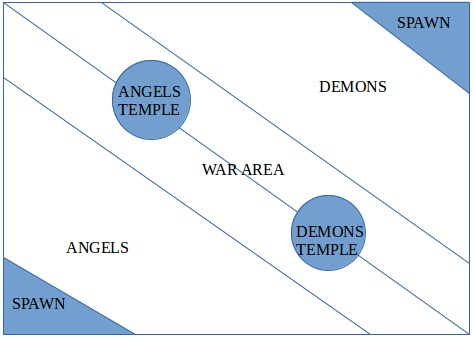
\includegraphics[width=0.7\textwidth]{outline.jpg}
\caption{\label{fig:outline}Bare outline of the map}
\end{figure}


\begin{enumerate}
\item Our game revolves around two teams Angels and Demons.

\item Each team will have its own team area on either side of the diagonal as shown in Figure. 1. The other team is not allowed to enter this area.

\item There is a common war area around the diagonal that both teams are allowed to enter.

\item The common war area around the diagonal will also have strategically located temples for each team.

\item There are 2 players per team. Therefore in total four players are allowed in MultiPlayer mode of the game.

\item The enemy team's team area is never visible.

\item The team's health is represented by the temple's health in the game. Destroying the enemy's temple means reducing enemy temple's health to zero.

\item Each player is assigned a hero. Each hero has his own health. Killing a hero means reducing it's health to zero. A hero is reborn after death in the team’s spawn area.

\item A team's temple health is considerably greater than it's individual hero's health.

\item The team area and war area will have obstacles(stones/trees) located. The hero will have to find paths around these obstacles to their target locations.

\item Each hero is allowed to move in horizontal and vertical direction. Once a target location is identified, the hero will use A* to reach the destination based on above restrictions.

\item The hero while traversing can pick certain items which add to its capabilities. The items are further described in the document.

\item Each hero will have a basic attacking capability and a magic power. Thus, each hero will have two modes of attack : Basic mode and Magic mode. Heros are further described in the document.

\item Each team will have it's own spawn area. A hero when born/re-born will find itself in this spawn area. Hero's can refuel their health by traversing back to this spawn area.
\end{enumerate}


\section{Play Modes}

We plan to offer two play modes for the end user. One being the \textbf{Bot Mode}, and other being the \textbf{MultiPlayer Mode}. In the \textbf{Bot Mode}, there will be one player with three AI players. The \textbf{MultiPlayer Mode} will allow four players on different nodes to play together, two players on each team.










\chapter{Screenshots}

\begin{figure}[htp]
\centering
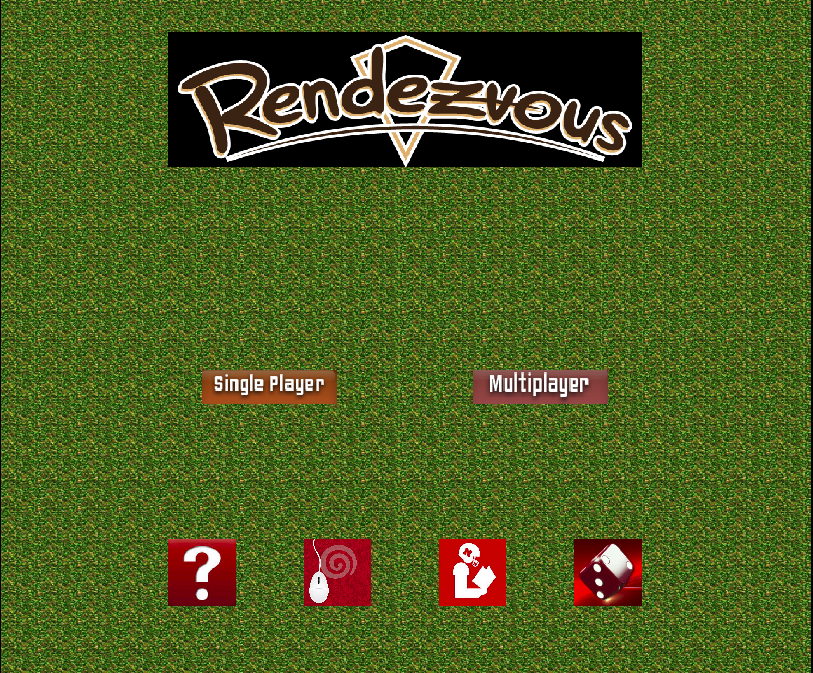
\includegraphics[width=1.1\textwidth]{Rendezvous.png}
\caption{\label{fig:start page}Rendezvous}
\end{figure}

\begin{figure}[htp]
\centering
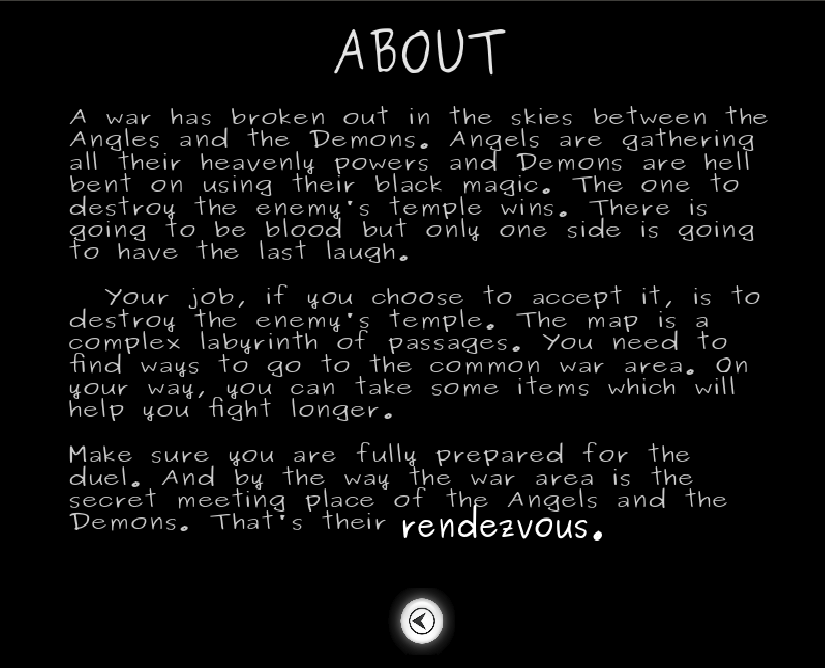
\includegraphics[width=1.1\textwidth]{About.png}
\caption{\label{fig:About}About Game}
\end{figure}

\begin{figure}[htp]
\centering
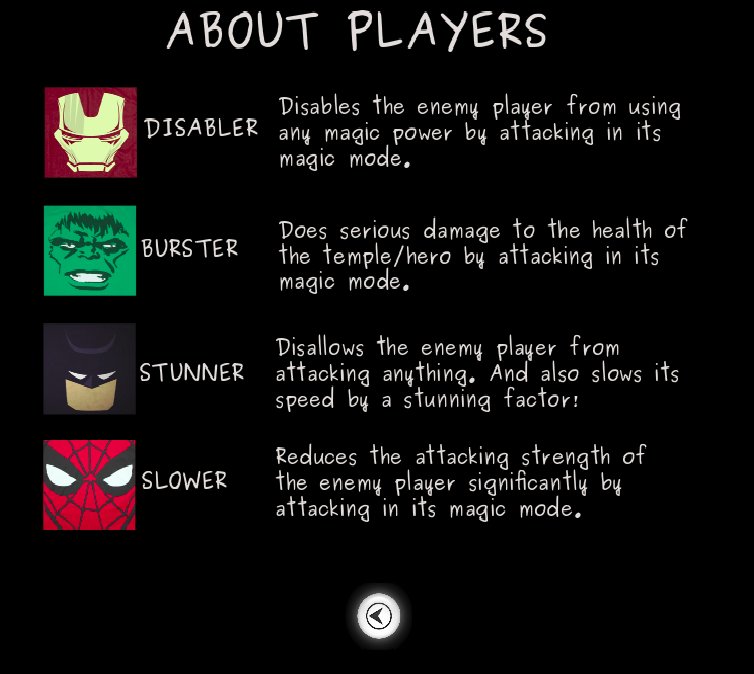
\includegraphics[width=1.1\textwidth]{About_players.png}
\caption{\label{fig:About_heroes}About Heroes}
\end{figure}

\begin{figure}[htp]
\centering
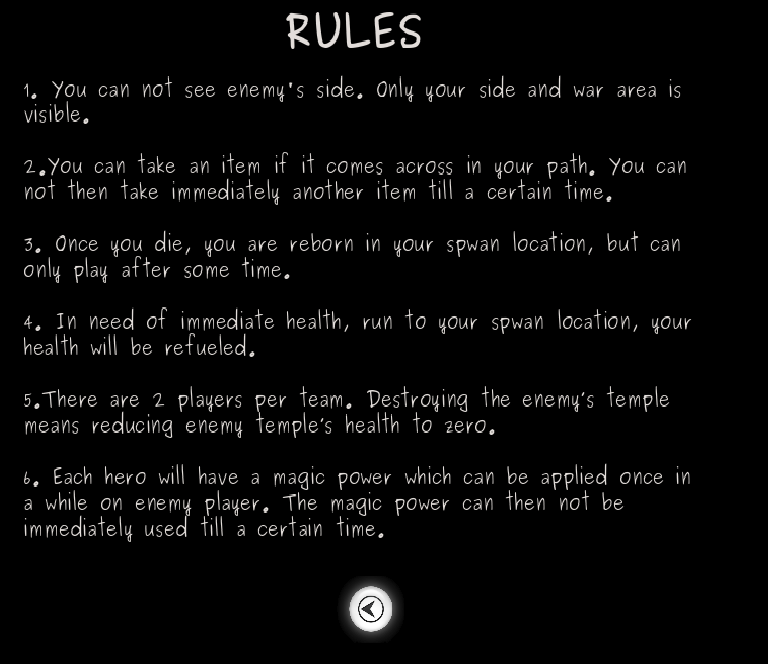
\includegraphics[width=1.1\textwidth]{Rules.png}
\caption{\label{fig:rules}Rules of the game}
\end{figure}

\begin{figure}[htp]
\centering
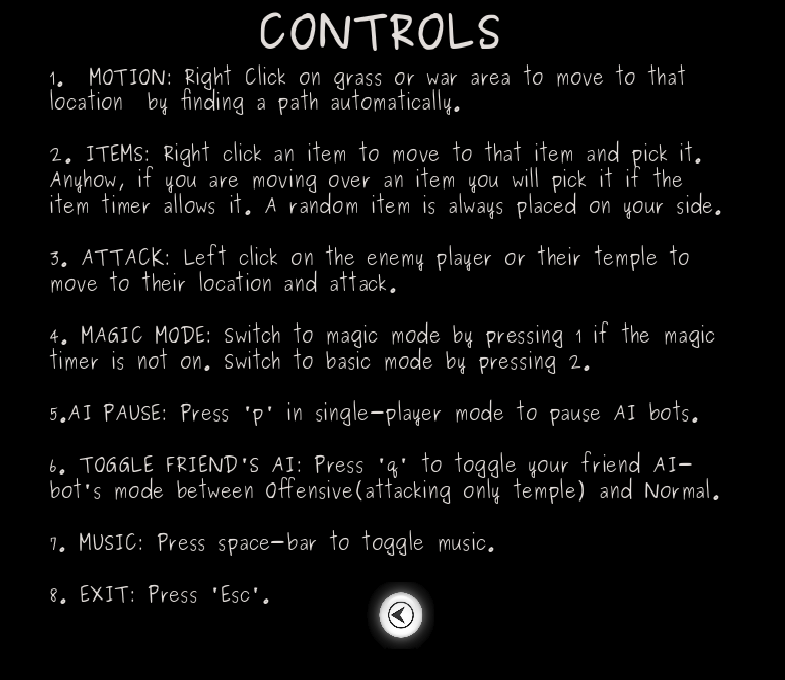
\includegraphics[width=1.1\textwidth]{Controls.png}
\caption{\label{fig:controls}Controls}
\end{figure}




\chapter{Map Details}

\section{Schematic Map Representation}
We have internally divided our map area into a grid of 20 by 20. Consider the schematic diagram of our map in Figure 2. We have represented the map details for one team in a table. The other team area has been left blank for it is a copy and paste mirror image of the same around the diagonal.

\begin{figure}[htp]
\centering
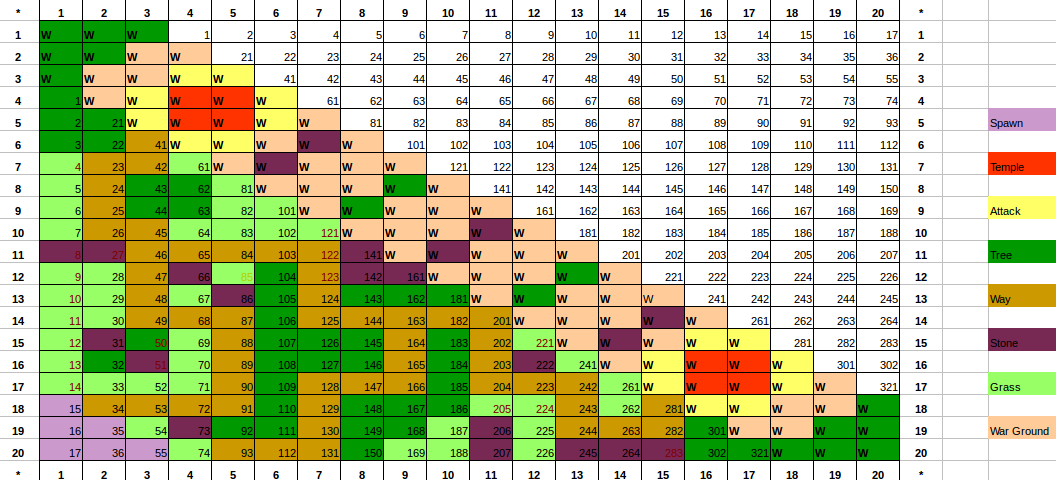
\includegraphics[width=1.1\textwidth]{Map_excel.png}
\caption{\label{fig:schematic}Schematic Map Representation}
\end{figure}


\section{Graphical Map Representation}
The graphical representation of our map respectively for both Demons and Angels is shown in Figure 3. Notice the visibility for both the teams. 

\begin{figure}[htp]
\centering
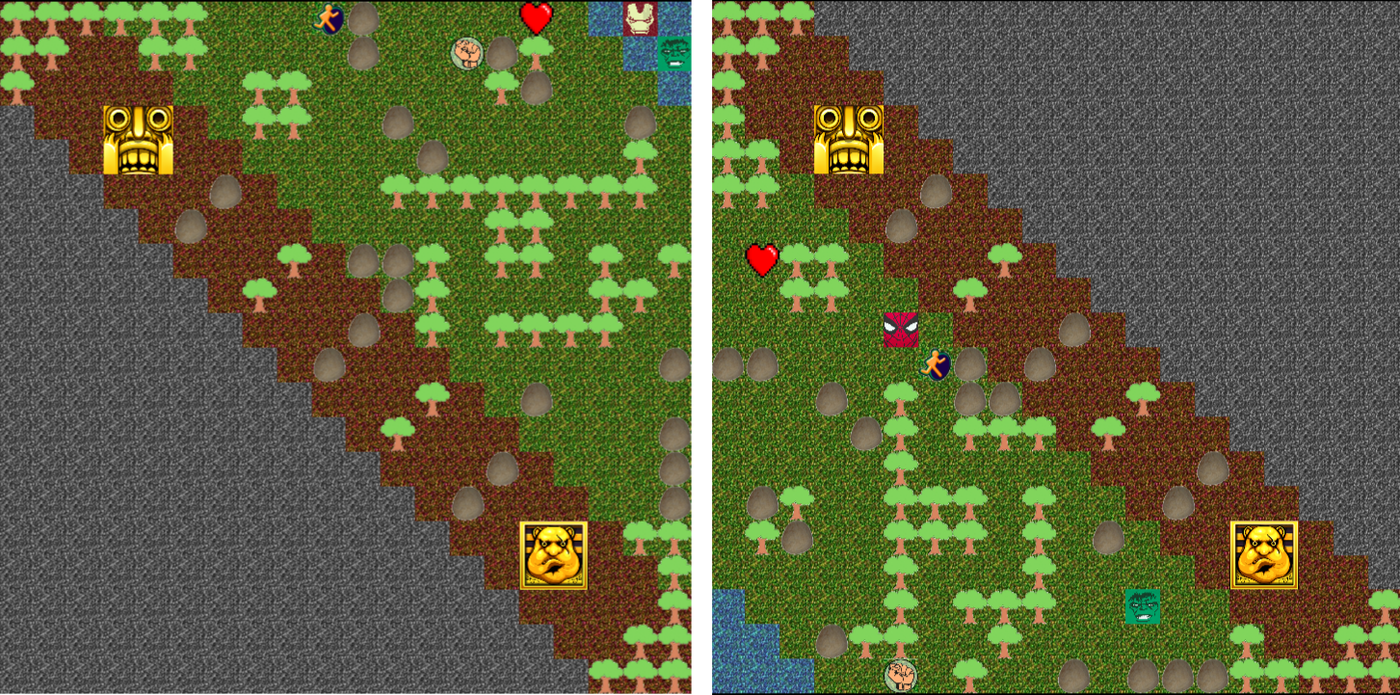
\includegraphics[width=1.0\textwidth]{Map_Views.png}
\caption{\label{fig:angels}Views of the Map}
\end{figure}


\section{Notification area}
The game is accompanied by an attribute area on both side of the maps, where the users can keep track of the game’s progress, etc. The schema for such an area is clearly depicted in Figure 4. 

\begin{figure}[htp]
\centering
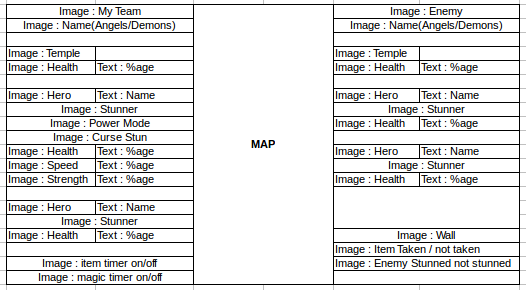
\includegraphics[width=0.9\textwidth]{attribute_space.png}
\caption{\label{fig:attribute}Schematic view of the attribute space}
\end{figure}


\section{Complete Map look}
The map in its entirety is shown in Figure 5. Notice the attribute area on either side.

\begin{figure}[htp]
\centering
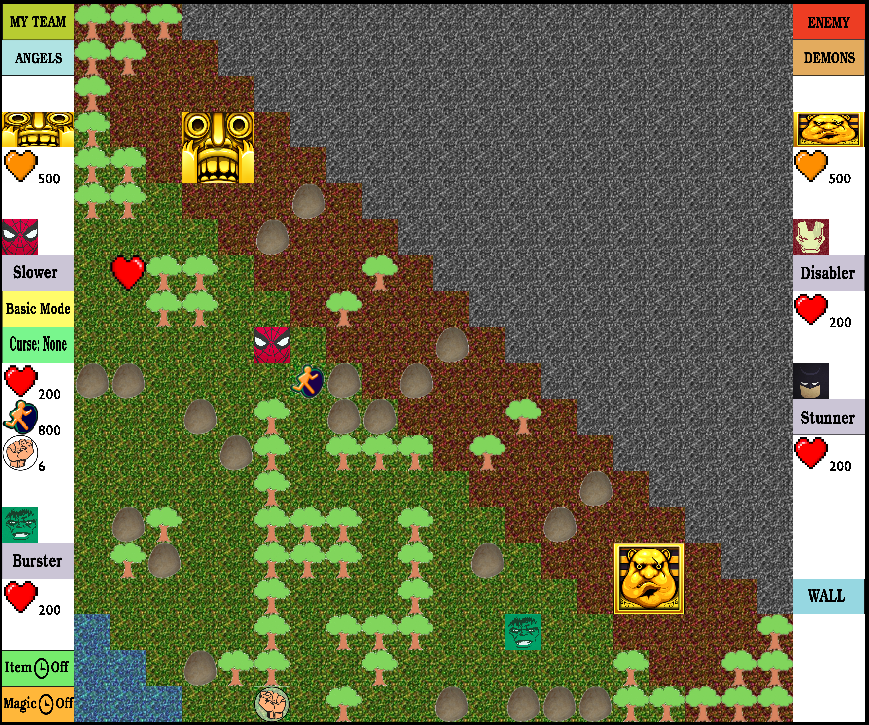
\includegraphics[width=0.7\textwidth]{Map_Attributes.png}
\caption{\label{fig:attributeMap}Complete Map with attribute space}
\end{figure}


\chapter{Game Attributes}

\section{Hero Details}
We have four heroes to play with as shown in Figure 6.\\

\begin{figure}[htp]
\centering
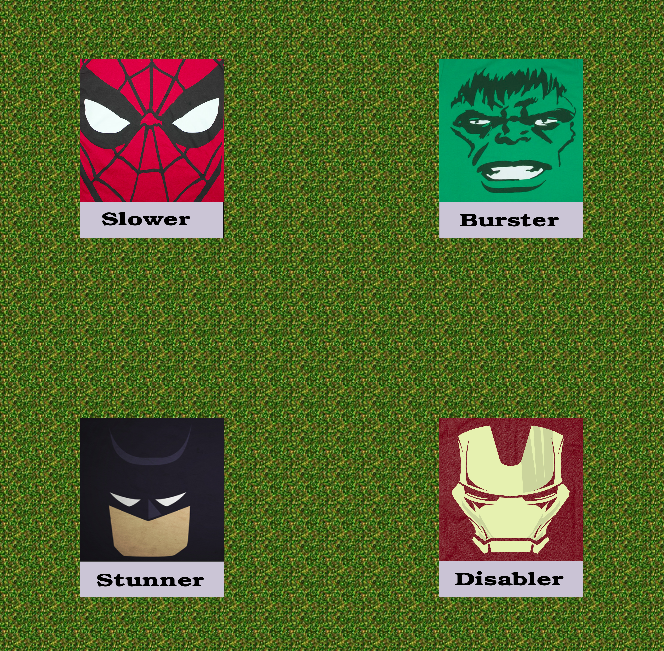
\includegraphics[width=0.5\textwidth]{Heros.png}
\caption{\label{fig:heroes}Heroes}
\end{figure}

Each hero has a unique magic power as described:
\begin{enumerate}
\item Stunner: Freezes the enemy player from attacking, moving, etc. for few seconds.
\item Slower: Reduces the attack capability of the enemy player for few seconds.
\item Disabler: Disables the enemy player from using any magical power for few seconds.
\item Burster: Does burst damage in a single shot.
\end{enumerate}

A hero is not allowed to use magic power in succession. It has to wait for some time before it can re-use the magic. \\

When a player uses it’s magic power on an enemy player, the enemy player is said to be cursed.

\section{Game Stats}
Each temple’s initial health is 500. Each hero’s initial heath is 200.
\\ \\
A hero has following attributes besides it’s health:
\begin{enumerate}
\item Strength: Damage done on a single attack
\item Speed: Movement speed (MIN 0 MAX 5)
\end{enumerate}

The above attributes depend on the hero type, as follows:
\begin{enumerate}
\item Stunner: Strength - 4, Speed - 2
\item Slower: Strength - 5, Speed - 2
\item Disabler: Strength - 6, Speed - 3
\item Burster: Strength - 7, Speed - 2
\end{enumerate}



\section{Item Details}
We have four items in our game. These items add to certain capabilities of the hero.
\begin{enumerate}
\item Speed Gain: Increases movement speed of the player by 1.
\item Strength Gain: Increases damage capability of the player by 2.
\item Temple Healer: Increases health of the player’s temple by 50.
\item Heath Gain: Increases health of the player by 20.
\end{enumerate}



\chapter{Running the game}

You can download the source code from ``https://github.com/abhiagar90/rendezvous". To build the code run `make' from the game directory.
You should have these commands already ran:
\begin{enumerate}
\item sudo apt-get install cmake
\item sudo apt-get install freeglut3-dev
\item sudo apt-get install mesa-common-dev
\item sudo apt-get install xorg-dev libglu1-mesa-dev
\item sudo apt-get install libpthread-stubs0-dev
\end{enumerate}

To install audio packages if needed in SoundAll.h, use the command : \\ ``sudo apt-get install libsfml-dev lsfml-audio'' \\

To run, after compiling the code, run `./a.out' from within the terminal in the current directory.



%\appendix
%\chapter{CHAPTER NAME}

\section{SECTION NAME}
\lipsum[1]

\section{SECTION NAME}
\lipsum[2]

\end{document}
	
